\chapter{Bevezetés}

A telefonok térnyerése az utóbbi évtizedben tagadthatatlan, életünk számos részét érintette,
illetve befolyásolta. Ezek alól nem képeznek kivételt a szabadidős elfoglaltságok, ezáltal
a horgászat sem. Ma már nehéz találni olyan horgászati tevékenységet végző embert, akinek a zsebében
ne lenne ott egy olyan telefon, amely minimum 50 milliószor több számítást végző kapacitással rendelkezik,
mint az 1962-ben létrehozott Apollo 11-es űrrakéta fedélzeti számítógépe \cite{realclearscience}. Több horgásztársamnak a fejében
is megfordult már, hogy akkor miért kell még mindig a fogásait papírra leírni, majd összegezni az év végén, 
és leadni azt a helyi horgász szövetségnél.

A rendszerváltás után rendszeresített fogási napló egy fontos problémát hivatott megoldani, ugyanis az 
egyre népszerűbb sport elfoglaltság veszélyeztette a hazai vizek halállományát, amiről ekkor még oly' keveset tudtunk.
Ez a rendszer volt hivatott arra a feladatra, hogy naplózzák, számon tartsák a kifogott halakat és összefüggéseket vonjanak le a hazai vizek élőlény állományáról.

\begin{figure}[h]
\centering
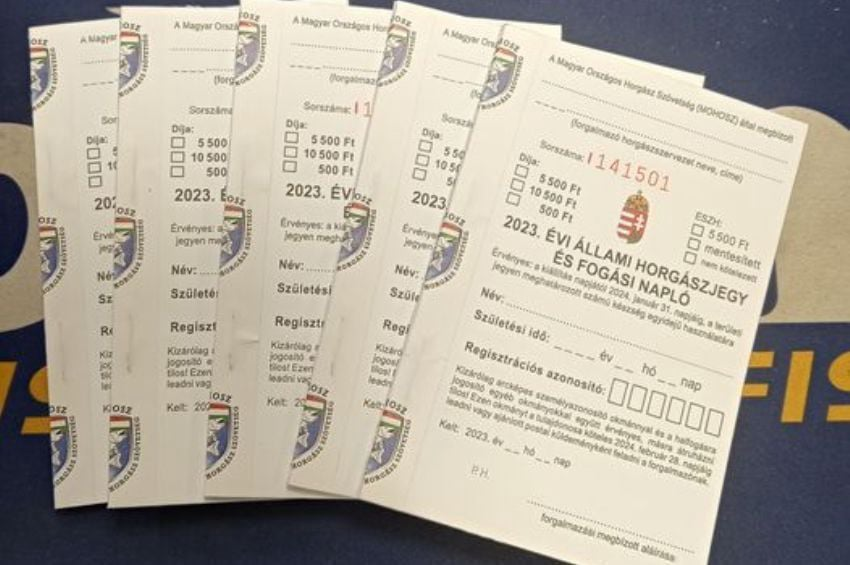
\includegraphics[scale=0.3]{images/fogasi_naplo.jpg}
\caption{2023. évi állami fogási naplók.}
\label{fig:fogasinaplok}
\end{figure}

Ezen a ponton találkozott a két kedvenc területem, a horgászat és a programozás. 
Az egyetemi éveim alatt szerteágazó tudásra tehettem szert, megismerhettem sokféle programozási nyelvet és
technikát. Külön kiemelném az adatbázis kezelést, és az objektum orientált programozási elvet, amelyek
nagy mértékben hozzásegítettek a szakdolgozati témám kiválasztásához, és megvalósításához.
Sokszor szó esett arról, hogy a programozás rengetegszer hétköznapi problémákat hivatott megoldani, ezáltal
könnyebbé tenni a felhasználó életét. 

Ezen a vonalon haladva határoztam el, hogy a szakdolgozati témám az állami fogási napló rendszer 
digitalizálása lesz. Ezzel az applikációval szeretném felhívni a figyelmet arra, hogy időleges
az előbbiekben említett rendszer átdolgozása, és a mai igényeket kielégítő okos telefonos integráció
létrehozása.

A továbbiakban be fogom mutatni, hogy az én elképzelésem alapján hogyan valósítható meg egy Androidos alkalmazás
Android Studio fejlesztői környezetben. Célja az alkalmazásnak, hogy felhasználó barát módon segítse horgásztársaimat a hétvégi kikapcsolódás során gyűjtött adatok - például a fogott halak súlya, a fogás pontos helye és időpontja - rögzítésére, és rendszerezésére. Az applikáció ezen túl segít a régebben rögzített fogások 
visszakeresésére, és áttekintésére. Kiemelt szempont volt az, hogy kezdő telefon felhasználók, ezáltal
az idősebb, okostelefont kevésbé használni tudók is könnyen és gyorsan használatba vehessék az alkalmazást. 
Törekedtem arra, hogy a program kezelői felülete a lehető legegyszerűbb, és átlátható legyen.

\begin{figure}[h]
\centering
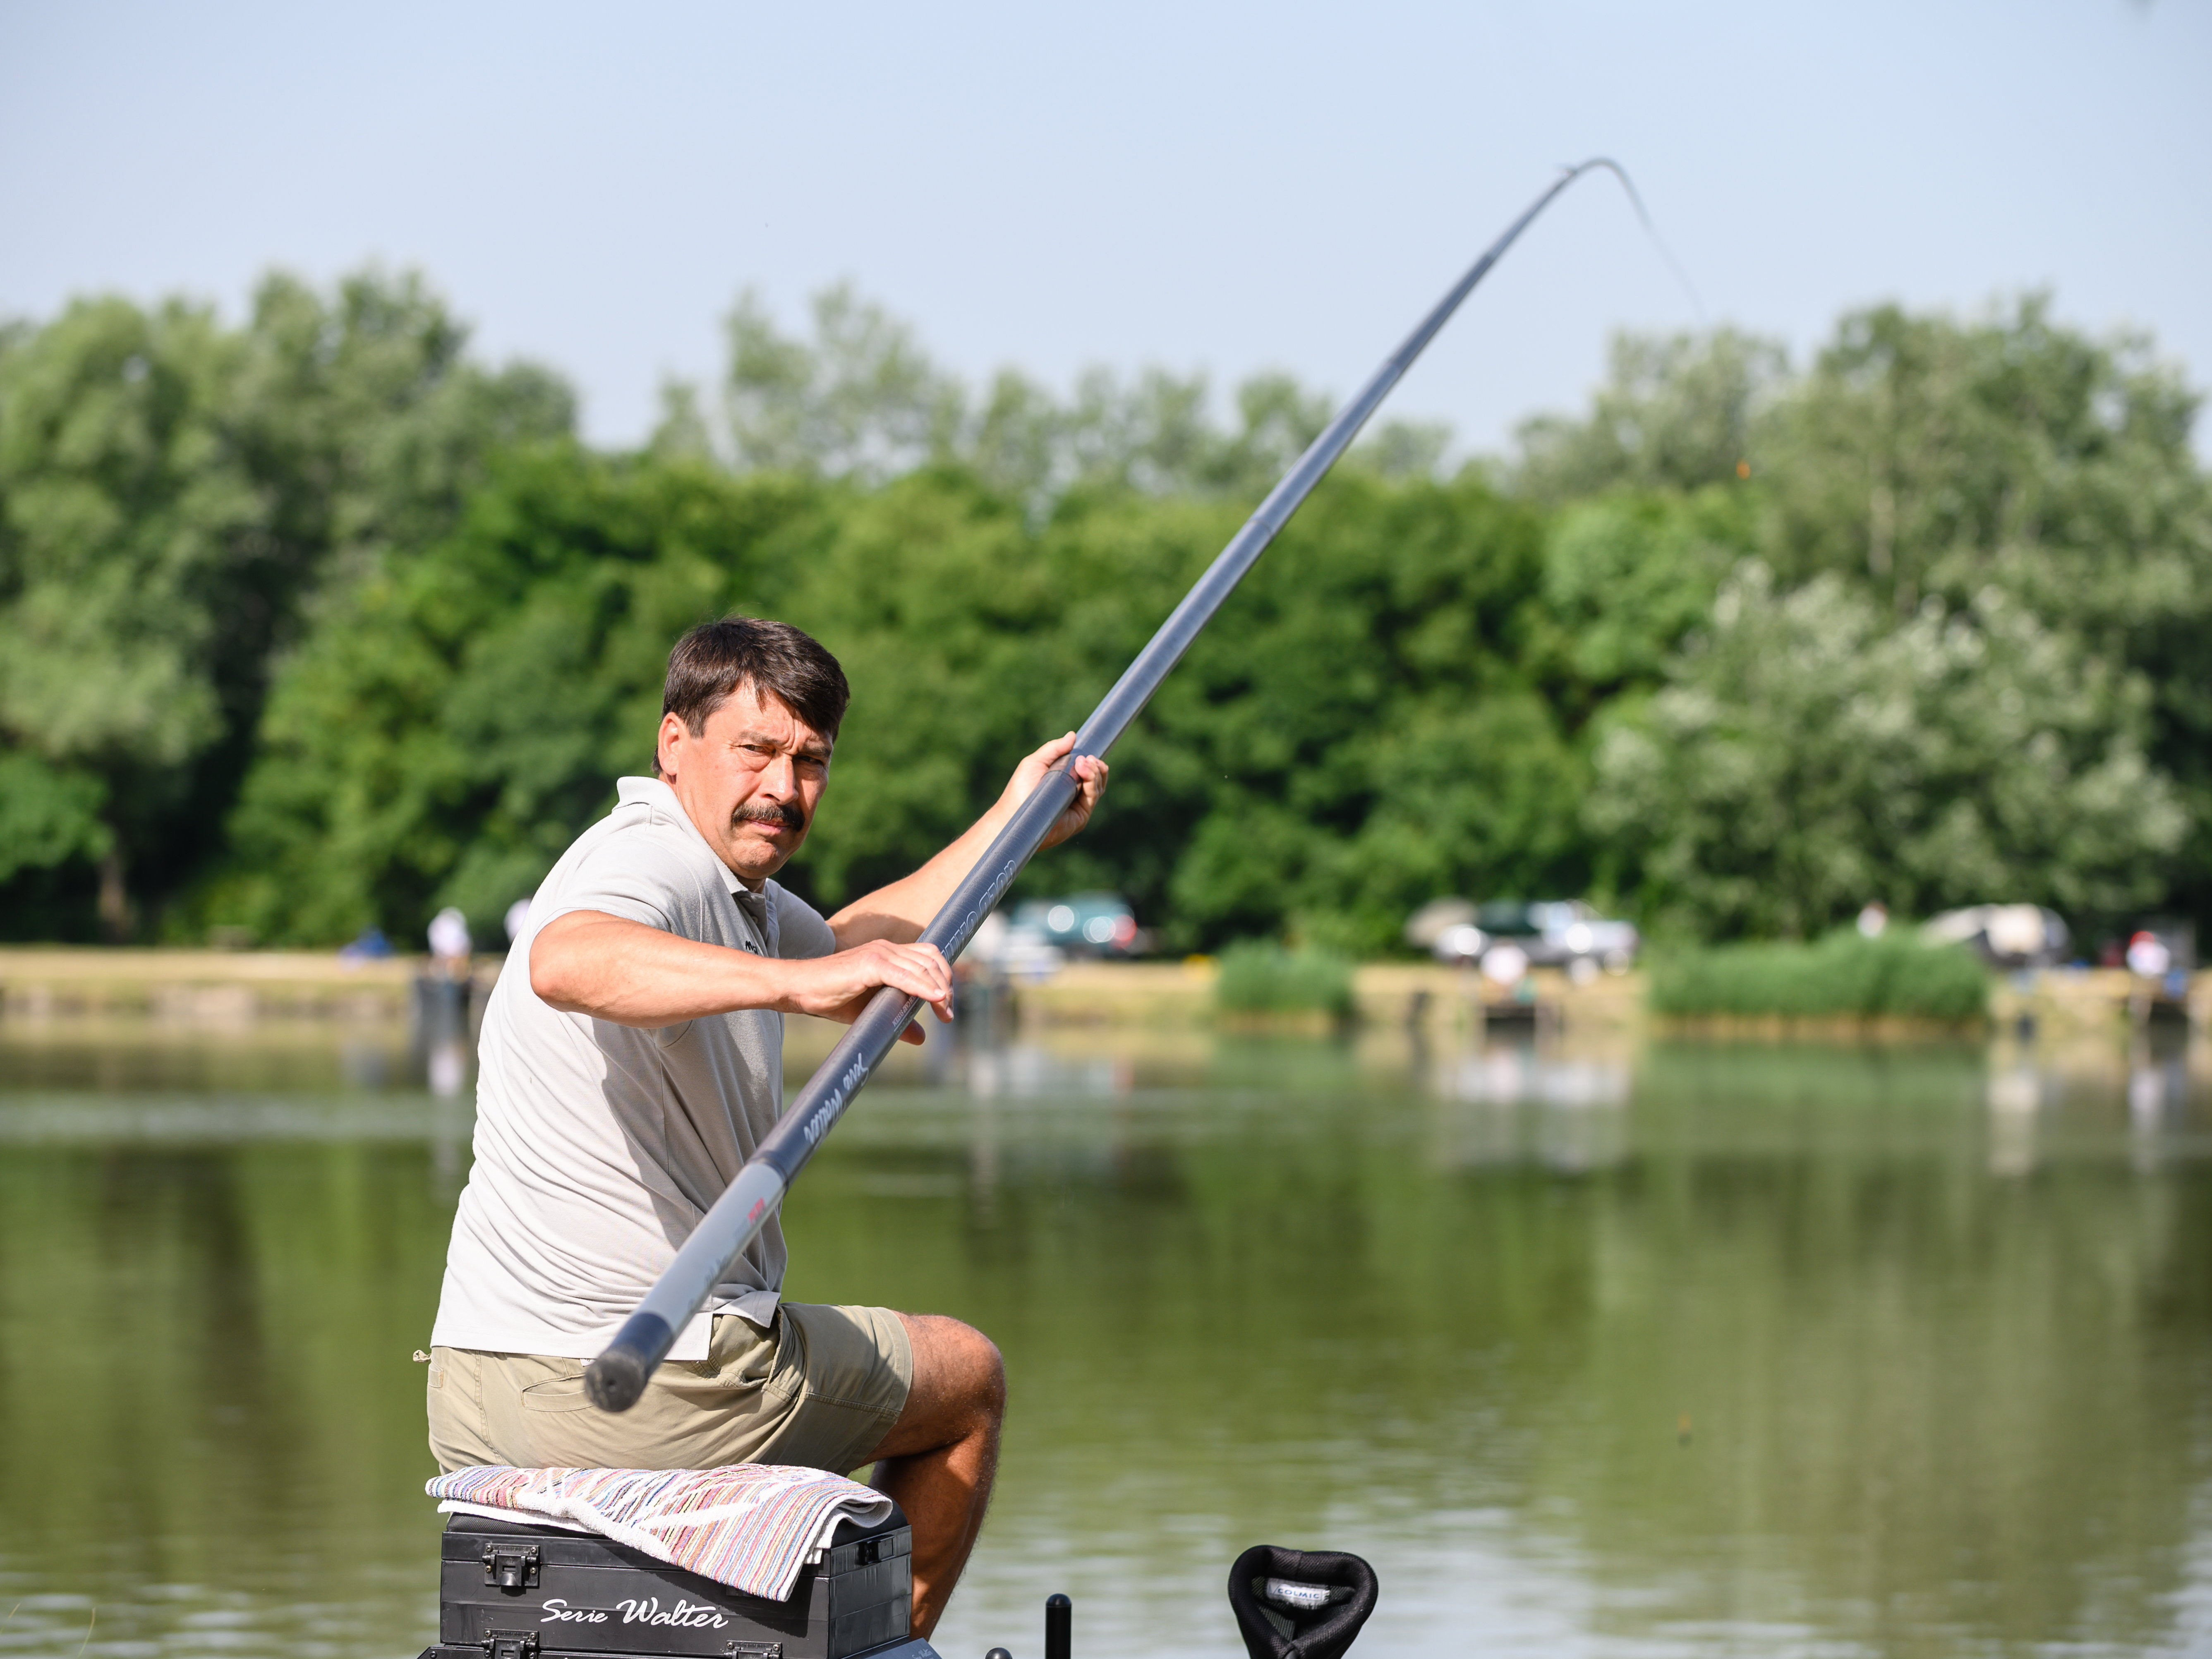
\includegraphics[scale=0.2]{images/horgaszat.jpg}
\caption{Horgászati tevékenységet végző ember.}
\label{fig:horgasz}
\end{figure}

A dolgozat az alábbi felépítést követi: az első fejezet bevezeti az olvasót a jelenlegi piaci helyzetbe, és 
rámutat a hiányosságokra, majd egy lehetséges megoldást nyújt. A második fejezet a fejlesztéshez szükséges 
technológiai alapokat, különösen az Android Studio és a hozzá kapcsolódó eszközök használatát mutatja be. A 
harmadik fejezet az alkalmazás architektúráját és a funkciók részletes leírását tartalmazza, míg a negyedik 
fejezet az alkalmazás megvalósításának módszereit tárgyalja. Az ötödik fejezet a tesztelési fázist mutatja be,
az utolsó fejezet pedig összefoglalja a projekt eredményeit, és javaslatokat fogalmaz meg a jövőbeni fejlesztésekre.